\documentclass[11pt]{article}

\usepackage{graphicx}
\newcommand{\head}[1]{\textnormal{\textbf{#1}}}
\begin{document}
    \begin{titlepage}
    \title {Design Document}
    \maketitle
        \begin{center}
		SE 2XA3\\
		\author{
		Hui Chen\hspace{128pt}chenh43	
		\\*Nareshkumar Maheshkumar\hspace{35pt}maheshn 
		\\*Sam Hamel\hspace{118pt}hamels2 \\
		}
		\end{center}
    \end{titlepage}
    
    \newpage
    
    \tableofcontents
    \listoffigures
    \listoftables
    
    \newpage
    \section{Revision History}
    \begin{table}[h]
    \caption{Revision History}
    \begin{tabular}{p{4cm}p{2cm}p{2cm}p{4cm}}
    Revision & Date & Team Member & Description of Change\\
    \hline
    0 & November 2 & Hui Chen & Started Design Document\\
    \hline
    0 & November 4 & Sam Hamel & Design Document Revision 0 Finished \\
    \hline
    0 & November 4 & Nareshkumar Maheshkumar & Edit and Proofread Revision 0\\
    \hline
    1 & November 6 & Hui Chen & Update MIS Section\\
    \hline
    1 & November 6 & Nareshkumar Maheshkumar & Design Document Revision 1 Finished\\
    \hline
     1 & November 6 & Sam Hamel & Edit and Proofread Revision 1\\
    \hline
    \end{tabular}
    \end{table}
    \newpage
    \section{Module Guide For No Limit Texas HoldEm Program(NLTP)}
    \subsection{Introduction}
    No Limit Texas HoldEm program follows model decomposition based on the principle of information hiding laid out by Parnas. The system is designed to be adaptable because possilbe future changes have been accounted for in the form of secrets. This flexibility will allow for easy revision control and will allow developers to quickly modify the program as needed. This design document includes in it a module guide (MG) of the system which gives a brief overview of the modules and allows both designers and maintainers to easily identify the parts of the software. The MG directly relates to the SRS with each requirement being fulfilled by either one module or the conjuction of several modules. For greater detail of the modules and what is needed to implement them there is the Module Interface Specifications (MIS), while the shedule of when these modules will be implemented is included in the Gantt and Pert charts.
    \subsection{Anticipated and Unlikely Changes}
    \subsubsection{Anticipated Changes}
    \textbf{AC1:} The specific hardware on which the software is running\\
    \textbf{AC2:} The algorithm used for hand ranking\\
    \textbf{AC3:} The deck shuffling algorithm\\
    \textbf{AC4:} The card distribution methods\\
    \textbf{AC5:} The pot/chip distribution methods\\
    \textbf{AC6:} AIOpponent chip betting methods\\
    
     
    \subsubsection{Unlikely Changes}
    \textbf{UC1:} Input/Output devices (Input: File and/or Mouse, Output: File, Memory, and/or Screen).\\
    \textbf{UC2:} The algorithm to calculate hand strength will always use the input from player’s hand and community card\\
    \textbf{UC3:} The game will always end when a player runs out of chips\\
    \textbf{UC4:} Any change to game state are always display to output devices\\
    \textbf{UC5:} Algorithm used to calculate AIOpponent’s action are defined using the parameters defined in the player and pot module\\
    
    \section{Module Hierarchy}
    This section provides an overview of the module design. Modules are summarized in a hierarchy decomposed by secrets in Table 1. The modules listed below, which are leaves in the hierarchy tree, are the modules that will actually be implemented.\\
    \textbf{M1: TexasHoldEm}\\
    \textbf{M2: Pot}\\
    \textbf{M3: Game}\\
    \textbf{M4: Hand}\\
    \textbf{M5: Deck}\\
    \textbf{M6: Player}\\
    \textbf{M7: AIOpponen}\\
    \textbf{M8: Card}\\
    \begin{table}[h]
    \caption{Module Hierarchy}
    \begin{tabular}{p{4cm}p{5cm}}
    \head{Level 1} & \head{Level 2} \\
    \hline
    Hardware Hiding & \\
    \hline
    Behaviour-Hiding  & TexasHoldEm Module \\
    Module & Pot Module\\
     & Game Module\\
    \hline
    Software Decision & Hand Module  \\
     & Deck Module\\
     & Player Module \\
     & AIOpponent Module\\
     & Card Module\\
    \hline
    \end{tabular}
    \end{table}
	
	\section{Connection Between Requirements and Design}
    The design of the system is intended to satisfy the requirements specified in the SRS. The system is decomposed into modules, and the connection between requirements and modules is listed in Table 3.
	\section{Module Decomposition}    
    \subsection{Hardware Hiding Module}
    Services: Includes programs that provide externally visible behavior of the system as specified in the software requirements specification (SRS) documents. This module serves as a communication layer between the hardware-hiding module and the software decision module. The programs in this module will need to change if there are changes in the SRS. \\
    Secrets: The contents of the required behaviors. \\
    Implemented By: –\\
    \subsubsection{Texas Holdem Module}
    Services: Displays GUI\\

    Secrets: GUI implementation\\

    Implemented by: NLTP\\

    \subsubsection{Pot Module}
    Services: Keeps track of chips in pot, and distributes chips to players\\

    Secrets: Method of distributing chips\\ 

    Implemented by: NLTP\\

    \subsubsection{Game module}
    Services: Manages the state of the game\\
    Secrets: How the game transitions between states \\
    Implemented by: NLTP\\

    \subsection{Behaviour-Hiding Module}
    Services: Includes data structure and algorithms used in the system that do not provide direct interaction with the user. \\
    Secrets: The design decision based on mathematical theorems, physical facts, or programming considerations. The secrets of this module are not described in the SRS. \\
    Implemented By: –\\

    \subsubsection{Hand Module}
    Services: Keeps track players’ cards, and calculates hand ranking\\

    Secrets: Algorithm for calculating ranking of cards \\

    Implemented by: NLTP\\

    \subsubsection{Deck Module}
    Services: stores, shuffles and distributes cards\\
    Secrets: Method of card distribution\\
    Implemented by: NLTP\\

    \subsubsection{Player Module}
    Services: let’s user fold/bet\\

    Secrets: Method of betting/folding\\

    Implemented by: NLTP\\

    \subsubsection{AIOpponnent Module}
    Services: Let’s AI fold/bet\\

    Secrets: Algorithm for calculating whether to bet/fold\\

    Implemented by: NLTP\\

    \subsubsection{Card Module}
    Services: object that represents playing cards\\

    Secrets: Card Contructor\\

    Implemented by: NLTP\\

    \subsection{Software Decision Module}
    
    \section{MIS of TexasHoldEm Module}
    
    \subsection{Exported Access Programs}
    \begin{table}[h]
    \caption{Exported Access Programs for TexasHoldEm Module}
    \begin{tabular}{p{4cm}p{2cm}p{2cm}p{4cm}}
    Name & In & Out & Exceptions\\
    \hline
	displayError() & int & - & Exception*\\
	\hline
    paint() & Graphic & - & -\\
    \hline
    save() & - & text file & FileNotFoundException\\
    \hline
    load() & text file & - & FileNotFoundException\\
    \hline
    actionPerformed() & ActionEvent &  - & - \\
    \hline
    \end{tabular}
    * all possible exceptions will be included, including but not limited to, FileNotFoundException and NullPointerException
    \end{table}
    
    \subsection{Interface Semantics}
    \subsubsection{State Variables}
    
    \subsubsection{Environment Variables}
	path:Location of the directory to be searched for when saving or loading the save file
	imagePath: Location of the directory to be searched for images of cards
    \subsubsection{Assumption}
    load() cannot be called without save() being called once before
    \subsubsection{Access Program Semantics}
    Main will populate the game window by instantiating the frame that is within TexasHoldEm module which will add all the components such as buttons, and uses paint() to populate the window with image of cards from environment variable imagePath and other simple graphics and colour for background. The save() will look for a save file in path. If it exists, it will overwrite it, if not, save() will create a new file. Load() will look for a save file in path and load all necessary data into the game and use Game module to modify the data for the affected modules. actionPerformed() will read the button input and call methods within Pot module based on its corresponding button. \\
    displayError():\\
    \textbf{Input} - Parameter of int type\\
    \textbf{transition} - Displays an error corresponding to the input  
    \newline
     \section{MIS of Pot Module}
     
    \subsection{Exported Access Programs}
    \begin{table}[h]
    \caption{Exported Access Programs for Pot Module}
    \begin{tabular}{p{4cm}p{2cm}p{2cm}p{4cm}}
    Name & In & Out & Exceptions\\
    \hline
    anti() & - & - & -\\
    \hline
    call() & - & - & -\\
    \hline
    raise() & int & - & -\\
    \hline
    fold() & - & - & - \\
    \hline
    getBet() & - & int & NullPointerException\\
    \hline
    getPot() & - & int & -\\
    \hline
    roundEndEvaluate() & - & - & - \\
    \hline
    \end{tabular}
    \end{table}
    \subsection{Interface Semantics}
    \subsubsection{State Variables}
    pot:int\\
    bet:int\\
    player1:Player\\
    player2:Player
    \subsubsection{Environment Variables}
    \subsubsection{Assumption}
    \subsubsection{Access Program Semantics}
    anti uses the Player module to modify both players' chips and also modifies the state variable pot by the same amount taken from player's chips. Call() and raise() uses the Player module to modify corresponding player's chips by the amount read by TexasHoldEm module. Fold() uses the Game module to modify the corresponding playerFolded parameter and also uses Player module to modify the amount of chips lost or gained. roundEndEvaluate() uses Player module to modify the amount of chips and uses the Game module to initialize a new round. \\
    getPot():\\
    \textbf{Input} - No input required\\
    \textbf{Output} - Returns the value corresponding to the parameter pot\\
    getBet():\\
    \textbf{Input} - No input required\\
    \textbf{Output} - Returns the value corresponding to the parameter bet
    \newline
     \section{MIS of Game Module}
     
    \subsection{Exported Access Programs}
    \begin{table}[h]
    \caption{Exported Access Programs for Game Module}
    \begin{tabular}{p{4cm}p{2cm}p{2cm}p{4cm}}
    Name & In & Out & Exceptions\\
    \hline
    playerSwitch() & - & - & -\\
    \hline
    deal() & - & - & -\\
    \hline
    nextCard() & - & - & -\\
    \hline
    isEndGame() & - & boolean & -\\
    \hline
    roundEnd() & - & - & - \\
    \hline
    player1Folded() & - & boolean & - \\
    \hline
    player2Folded() & - & boolean & - \\
    
    \end{tabular}
    \end{table}
    \subsection{Interface Semantics}
    \subsubsection{State Variables}
    currentPlayer:int\\
    Deck: list of Cards\\
    player1: Player\\
    player2: Player\\
    endGame: boolean\\
    player1Fold: boolean\\
    player2Fold: boolean
    \subsubsection{Environment Variables}
    \subsubsection{Assumption}
    \subsubsection{Access Program Semantics}
 	roundEnd() will call upon methods in Pot to evaluate, distribute the pot to the players and modify the parameters Deck, endGame, currentPlayer and each Player's hand by initializing the corresponding parameters as their default value or distribute new cards to the players.\\
 	playerSwitch():\\
 	\textbf{Input} - No input required\\
 	\textbf{transition} - modify currentPlayer between 2 values\\
 	deal():\\
 	\textbf{Input} - No input required\\
 	\textbf{Output} - Populates the Player hand variable\\
 	nextCard():\\
 	\textbf{Input} - No input required\\
 	\textbf{Output} - Modifies both players' hands by adding the same additional card to each hand\\
 	isEndGame():\\
 	\textbf{Input} - No input required\\
 	\textbf{Output} - boolean value corresponding to the value of parameter endGame\\
 	player(1/2)Folded():\\
 	\textbf{Input} - No input required\\
 	\textbf{Output} - boolean value corresponding to the value of their respective parameters
 	\newline 
 	
 	\section{MIS of Deck Module}
     
    \subsection{Exported Access Programs}
    \begin{table}[h]
    \caption{Exported Access Programs for Deck Module}
    \begin{tabular}{p{4cm}p{2cm}p{2cm}p{4cm}}
    Name & In & Out & Exceptions\\
    \hline
    setDeck() & - & - & - \\
    \hline
    Shuffle() & - & Deck & -\\
    \hline
    \end{tabular}
    \end{table}
    \subsection{Interface Semantics}
    \subsubsection{State Variables}
	Deck: list of cards    
    \subsubsection{Environment Variables}
    \subsubsection{Assumption}
    Card module is created before Deck module
    \subsubsection{Access Program Semantics}
    setDeck:\\
    \textbf{Input} - No input required\\
    \textbf{Output} - Populates the Deck with Cards\\  
    Shuffle:
    \textbf{Input} - No input required\\
    \textbf{Transition} - Modifies the Deck so that it is randomized\\
 	\newline
 	\section{MIS of Card Module}
    
    \subsection{Exported Access Programs}
    \begin{table}[h]
    \caption{Exported Access Programs for Card Module}
    \begin{tabular}{p{4cm}p{2cm}p{2cm}p{4cm}}
    Name & In & Out & Exceptions\\
    \hline
    getRank() & - & int & DNE\\
    \hline
    getSuit() & - & char & DNE\\
    \hline
    \end{tabular}
    \end{table}
    \subsection{Interface Semantics}
    \subsubsection{State Variables}
    rank:int\\
    suit:char
    \subsubsection{Environment Variables}
    \subsubsection{Assumption}
    \subsubsection{Access Program Semantics}
    Get: \\
    \textbf{Input} - No input required\\
    \textbf{Output} - return value of corresponding parameter\\
 	\newline
 	\section{MIS of Player Module}
     
    \subsection{Exported Access Programs}
    \begin{table}[h]
    \caption{Exported Access Programs for Player Module}
    \begin{tabular}{p{4cm}p{2cm}p{2cm}p{4cm}}
    Name & In & Out & Exceptions\\
    \hline
    getChips() & - & - & -\\
    \hline
    gainChips() & int & - & -\\
	\hline    
    loseChips() & int & - & EMPTY\\
	\hline    	
    getHand() & - & Hand & NullPointerException \\
	\hline    
    setHand()& Hand & - & -\\
    \hline
    \end{tabular}
    \end{table}
    \subsection{Interface Semantics}
    \subsubsection{State Variables}
    chips:int\\
    Hand: list of Cards
    \subsubsection{Environment Variables}
    \subsubsection{Assumption}
    getHand() can only be called after setHand()
    \subsubsection{Access Program Semantics}
    Get:\\
    \textbf{Input} - No input required\\
    \textbf{Output} - Each Get method will return value of the corresponding parameter\\
    setHand:\\
   	\textbf{Input} - Input will take parameter Hand\\
   	\textbf{Transition} - Modifies the state of Hand\\
   	(gain/lose)Chips:\\
   	\textbf{Input} - Input will take parameter of int type\\
   	\textbf{Transition} - Modifies the state of chips
 	\newline
 	\section{MIS of AIOpponent Module}
     
    \subsection{Exported Access Programs}
    \begin{table}[h]
    \caption{Exported Access Programs for AIOpponent Module}
    \begin{tabular}{p{4cm}p{2cm}p{2cm}p{4cm}}
    Name & In & Out & Exceptions\\
    \hline
    getAction() & - & - & -\\
    \hline
    \end{tabular}
    \end{table}
    \subsection{Interface Semantics}
    \subsubsection{State Variables}
    \subsubsection{Environment Variables}
    \subsubsection{Assumption}
    getAction is only called when it gets to its turn in the Game module
    \subsubsection{Access Program Semantics}
    getAction will determine the move the AI will take by evaluating the current state of the board and its current Hand, and will call upon the Game module for its action. 
    \newline
    \section{MIS of Hand Module}
    \subsection{Exported Access Programs}
    \begin{table}[h]
    \caption{Exported Access Programs for Hand Module}
    \begin{tabular}{p{4cm}p{2cm}p{2cm}p{4cm}}
    Name & In & Out & Exceptions\\
    \hline
    evaluate() & Hand & int & -\\
    \hline
    getStrength() & - & int & -\\
    \hline
    myHand() & - & String & - \\
    \hline
    \end{tabular}
    \end{table}
    \subsection{Interface Semantics}
    \subsubsection{State Variables}
    hand: list of Cards\\
    strength: int
    \subsubsection{Environment Variables}
    \subsubsection{Assumption}
    evaluate() is only called when roundEnd() or player1Folded() or player2Folded() from game is called.
    \subsubsection{Access Program Semantics}
    getStrength():\\
    \textbf{Input} - No input required\\
    \textbf{Output} - Returns value of parameter strength\\
    myHand():\\
    \textbf{Input} - No input required\\
    \textbf{Output} - Returns the Cards in hand\\
    evaluate():\\
 	
    \section{Use Hierarchy}
    \begin{figure}[h]
		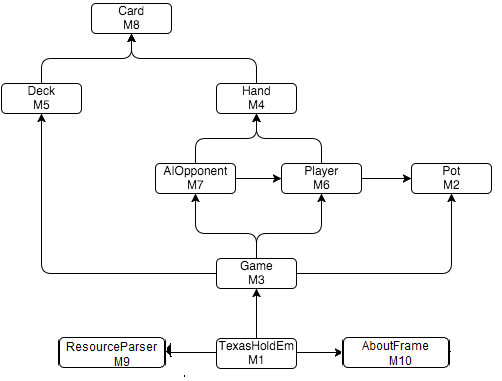
\includegraphics[scale=0.7]{Uses.png}
		\caption{Use Hierarchy Diagram}
		\label{fig1: Figure1}
		\end{figure}
    \section{Traceability Matrix}
    \begin{table}[h]
    \caption{Traceability Matrix Between the Module And Requirements}
    \begin{tabular}{p{4cm}p{2cm}p{2cm}p{4cm}}
    Requirements & Modules\\
    \hline
    R1 & N/A\\
    \hline
    R2 & M1\\
    \hline
    R3 & M2,M6,M7\\
    \hline
    R4 & M2,M3\\
    \hline
    R5 & M6,M7\\
    \hline
    R6 & M4,M8\\
    \hline
    R7 & M3\\
    \hline
    R8 & M2\\
    \hline
    R9 & M2\\
    \hline
    R10 & M2,M3\\
    \hline
    \end{tabular}
    \end{table}
    
    \begin{table}[h]
    \caption{Traceability Matrix Between Anticipated Changes And Requirements}
    \begin{tabular}{p{4cm}p{2cm}p{2cm}p{4cm}}
    Anticipated Changes(AC) & Modules\\
    \hline
    AC1 & N/A\\
    \hline
    AC2 & M4\\
    \hline
    AC3 & M5\\
    \hline
    AC4 & M8\\
    \hline
    AC5 & M2\\
    \hline
    AC6 & M7\\
    \hline
    \end{tabular}
    \end{table}
    \newpage
    \section{Schedule}
        
    \end{document}